% mainfile: ../RobertoDiRemigioPhDThesis.tex
\chapter{Continuum Solvation Models}\label{ch:CSM}

\epigraph{
\textitalian{
L'acqua è la forza che ti tempra,

nell'acqua ti ritrovi e ti rinnovi:

noi ti pensiamo come un'alga, un ciottolo,

come un'equorea creatura

che la salsedine non intacca

ma torna al lito più pura.
}
}{
    --- \textsc{Eugenio Montale}, \textit{Falsetto}}

Developments of the \gls{PCM}, a continuum solvation model, are at the
heart of this thesis.
This Chapter is a brief exposition of the major points of the \acrshort{PCM}
we have worked upon in the thesis.
Appendix \ref{app:mathematical-results} contains much of the
mathematical details omitted from the exposition in this Chapter.
Section \ref{sec:IEF} will present the formulation of the model.
I will show how a variational approach can facilitate the formulation of
quantum/classical polarizable Hamiltonians in Section
\ref{sec:variational}.
Section \ref{sec:BEM} will be devoted to the numerical strategies used
in solving the \acrshort{PCM} equation.

Continuum models have a venerable history in quantum chemistry:
\citeauthor{Onsager1936-wf}'s model\autocite{Onsager1936-wf} appeared in
1936 and the first form of the \acrshort{PCM} entered the stage in
1981.~\autocite{Miertus1981-mm}
Section \ref{sec:CSM-why-how} will offer a heuristic "derivation" of
continuum models.
While it cannot be thought as formally rigorous, it highlights the major
physical insights that have informed the creation of continuum models.
Still nowadays much research activity is expended on the
\acrshort{PCM}.~\autocite{Tomasi2011-un, Mennucci2012-dv, Lipparini2016-mo}
I will point out throughout the Chapter to developments outside our
group that are particularly interesting.

\section{Continuum Solvation Models: Why and How}\label{sec:CSM-why-how}

The basic idea of implicit models is that the environment can
be replaced by a structureless continuum.
The continuum will interact \emph{classically} with the explicit part of
the multiscale model, an interaction mediated by some macroscopic
property of the bulk material the continuum represents.
Thus, continuum models bypass both problems plaguing explicit models we
mentioned in the Introduction, namely:
\begin{enumerate*}[label={\alph*)},font={\color{PMS1797}}]
\item the statistical averaging of environment configurations and
\item the \acrshort{MM} region electrostatics cutoff choice.
\end{enumerate*}

Following \citeauthor{Tomasi2007-es}, we introduce the complete system
Hamiltonian in the \acrshort{BO} approximation:~\autocite{Tomasi2004-dc,
Tomasi2007-es}
\begin{equation}\label{eq:solution-ham}
 H(\vect{r}_\mathrm{S}, \vect{r}_\mathrm{E}) =
  H_\mathrm{S}(\vect{r}_\mathrm{S}) +  H_\mathrm{E}(\vect{r}_\mathrm{E})
+ H_\mathrm{SE}(\vect{r}_\mathrm{S}, \vect{r}_\mathrm{E})
\end{equation}
The Hamiltonian features solute terms, marked by the S subscript,
environment terms, marked by the E subscript, and interaction terms.
The coordinates $(\vect{r}_\mathrm{S}, \vect{r}_\mathrm{E})$ refer to
\emph{both} nuclei and electrons.
The interaction term is given by the usual Coulomb electrostatic
Hamiltonian.

One can replace the pure environment and interaction terms with their
classical counterparts and obtain the quantum/classical, possibly
\emph{polarizable}, Hamiltonian for an explicit \acrshort{QM}/\acrshort{MM} model.
This brings about the first important point: the need for statistical
averaging.
Whenever a large number of degrees of freedom is involved, one can
access macroscopic observables of the system by the appropriate
averaging of the microscopically detailed motion over phase space
trajectories or on the appropriate statistical
ensemble.~\autocite{Hill1960-ql}
The need for ensemble averages leads us to the following observations:
\begin{enumerate*}[label={\alph*)},font={\color{PMS1797}}]
 \item
   the need for \emph{macroscopic} parameters, absent from the
   microscopic Hamiltonian Eq.~\eqref{eq:solution-ham}, in carrying out
   statistical simulations.
 \item
   Chosen a thermodynamic ensemble, the basic energetic quantity is
   accordingly determined. For example, the Gibbs free energy  $G$ is
   intrinsically related to the $(NpT)$ ensemble.
 \item
   Even atomistic simulations will lead to results that are essentially
   averages. The discrete picture of the system has been replaced by
   some continuous distribution function.
\end{enumerate*}

These observations strongly suggest that one can perform the averaging
step \emph{before} embarking into the solution of the quantum mechanical
problem and replace the full Hamiltonian with and \emph{effective}
Hamiltonian in which the environment degrees of freedom are properly
averaged.~\autocite{Angyan1992-vo, Tapia1992-pu}
The solute-environment interaction term would then be replaced by
a term only depending on the solute degrees of freedom, represented by
the averaged, continuous response functions of the solvent.
This is the physical setting of the \gls{PCM} and is schematically
depicted in Figure \ref{fig:IEF}.
The solute molecule is enclose in a \emph{cavity} inside the
structureless continuum representing the solvent and the basic energetic
quantity is a \emph{free energy}:\autocite{Tomasi1994-gv,
Amovilli1998-pv, Tomasi2005-vm}
\begin{equation}\label{eq:free-energy}
 G = G_\mathrm{cav} + G_\mathrm{el} + G_\mathrm{dis} + G_\mathrm{rep} + G_\mathrm{Mm}(T).
\end{equation}
The decomposition of the solute free energy takes into account the
different physical origins of the different solute-solvent interactions.
$G_\mathrm{cav}$ is the cavity formation free energy, a constant as long
as the solute geometry does not change.\autocite{Tomasi1994-gv,
Floris1997-tu}
The second term $G_\mathrm{el}$ is the most important one in the
framework of continuum models. It accounts for the mutual electrostatic
polarization of solute and solvent, see Section \ref{sec:IEF}.
The third $G_\mathrm{dis}$ and fourth $G_\mathrm{rep}$ terms account for
dispersion and repulsion interactions,
respectively.\autocite{Amovilli1997-fo, Weijo2010-jy}
Finally, $G_\mathrm{Mm}(T)$ accounts for the collective molecular
motions of the solute-solvent system. It explicitly depends on the
temperature $T$ and can be calculated from the solution partition
function, see \noparcite[ref.][]{Amovilli1998-pv} for further details.

In this thesis, we focused exclusively on the purely electrostatic
component of the interaction energy, completely neglecting the other
terms.
While a balanced description of solvation chemistry certainly demands
a proper treatment of all solute-solvent interactions, especially when
non homogeneous environments are studied,\autocite{Mozgawa2014-ad,
Mozgawa2016-wf} it is also true that the electrostatic component is the
most numerically relevant and the most sensitive to changes in the
system studied and in the level of quantum mechanical description.

\begin{figure}[!h]
  \centering
  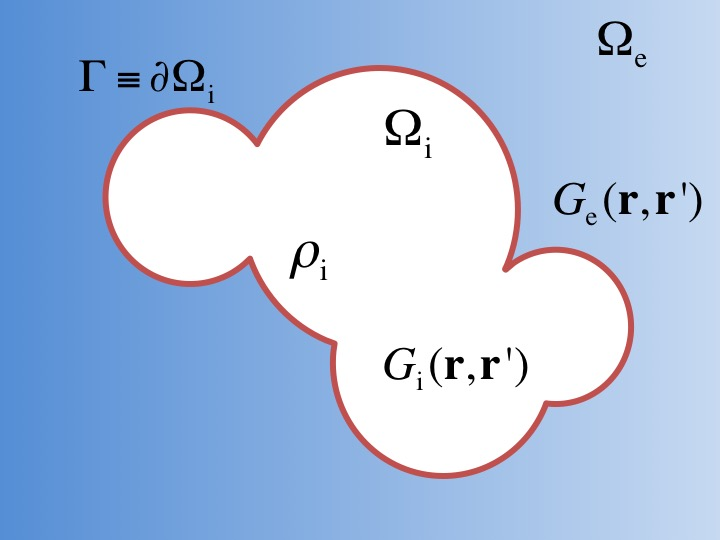
\includegraphics[width=.5\textwidth]{IEF}
  \caption[The physical setting of the polarizable continuum model.]{
  The physical setting of the \gls{PCM}. The molecular solute,
  represented by its, possibly quantum mechanical, charge density
  $\rho_\mathrm{i}$ is enclosed in a \emph{cavity} $\Omegai$.
  The boundary of the cavity $\Gamma\equiv\partial\Omegai$ is a
  continuously differentiable 2-manifold.
  We assume the material properties of the cavity to be those of vacuum,
  hence characterized by the Green's function
  $\Gi=\frac{1}{|\vect{r}-\vect{r}^\prime|}$.
  The cavity is carved out of an infinite, structureless, continuum
  characterized by its Green's function $\Ge$ and fully covering the
  external subdomain $\Omegae$.
  }
  \label{fig:IEF}
\end{figure}

\section{Continuum Electrostatics as a Boundary Integral Problem}\label{sec:IEF}

The molecular solute, represented by its charge density
$\rhoi$ is enclosed in a \emph{cavity} $\Omegai$.
The boundary of the cavity $\Gamma\equiv\partial\Omegai$ is a
2-manifold and is assumed to be continuously differentiable, \ie $\mathcal{C}^1$.
The cavity is carved out of an infinite, structureless, continuum
characterized by the bulk properties of the solvent.
The continuum fully spans the external subdomain $\Omegae$, see Fig. \ref{fig:IEF}.
The source charge density is not assumed to be continuous: both
classical point multipoles and quantum mechanical charge densities can
be treated within the model.
However, we assume that its support is entirely within the cavity,
$\Supp(\rhoi) \subseteq \Omegai$. This assumption is, of course, false
for quantum mechanical charge densities. It can however be proven that
the errors induced by this \emph{charge penetration} are not so
severe.~\autocite{Chipman2000-us, Cances2001-qs, Cances2001-qn}

Formulated as such, the \gls*{PCM} is a well-known problem in classical
electrostatics: find the electrostatic potential in space generated by
a charge distribution confined in a cavity in a \emph{polarizable}
continuous medium.\autocite{Jackson1999, Vanderlinde2005-gf}
In the mathematical literature on \acp{PDE}, it is usually referred to as a
\emph{transmission} problem.\autocite{Hackbusch1995-uq, Sauter2011-an}

Given the partition of Euclidean space $\mathbb{R}^3$ outlined above,
find the solution $u(\vect{r})$ to the following set:
\begin{subequations}\label{eq:transmission}
  \begin{align}[left={\empheqlbrace}]
  \Li u &= \nabla^2 u = -4\pi\rhoi \,\, \text{in}\,\, \Omegai \label{eq:internal} \\
  \Le u &= 0 \,\, \text{in}\,\, \Omegae \label{eq:external} \\
  [u] &= \ue - \ui = 0 \,\, \text{on}\,\, \Gamma
  \label{eq:trace-jump} \\
[\partial_L u] &= \partiale u - \partiali u = 0 \,\, \text{on}\,\, \Gamma \label{eq:conormal-jump} \\
|u(\vect{r})| &\leq C \|\vect{r} \|^{-1} \,\,\text{for}\,\,\| \vect{r} \|\rightarrow\infty
\label{eq:radiation}
\end{align}
\end{subequations}
Eqs.~\eqref{eq:trace-jump} and \eqref{eq:conormal-jump}
are the \emph{jump conditions}, expressed in terms of trace operators
for the solution $u$ and its \emph{conormal} derivative.
For notational simplicity, will use the symbols $\partiale$ and $\partiali$
for the latter and only give it in explicit form when needed.
Further mathematical details and technical results on the definition of
function traces and their use in setting up the proper normal and
conormal derivatives can be found in the excellent book by
\citeauthor{Sauter2011-an}.~\autocite{Sauter2011-an}.
The fundamental solutions, or Green's functions, for the elliptic
differential operators $\Li$ and $\Le$ will be denoted by $\Gi$ and
$\Ge$, respectively.
As such the problem is formulated in the so-called \emph{strong} form:
the sought-after solution $u$ has to be at least two times continuously
differentiable.
Moreover, the solution is a function supported over $\mathbb{R}^3$ which
poses challenges to the numerical solution of the problem.
We will take a different approach and reformulate it in terms of
\emph{boundary integral operators}, \ie transform the \acsp{PDE} into a
\gls{BIE}.

The first step is to introduce the relevant boundary integral operators for the
above mentioned transmission problem.
They are three of the four components of the Calder\'on projector.
For any function $v$ in the suitable function space and for $\vect{s}, \vect{s}^\prime \in \Gamma$:
\begin{subequations}
\begin{align}
  (\bi{S}_\star v)(\vect{s}) &= \int_\Gamma
  G_\star(\vect{s}, \vect{s}^\prime)v(\vect{s}^\prime)\diff
  \vect{s}^\prime \label{eq:S} \\
  (\bi{D}_\star v)(\vect{s}) &= \int_\Gamma \partial_{L_\star,\vect{s}}
  G_\star(\vect{s}, \vect{s}^\prime)v(\vect{s}^\prime)\diff
  \vect{s}^\prime \label{eq:D} \\
  (\bi{D}^\dagger_\star v)(\vect{s}) &= \int_\Gamma
\partial_{L_\star,\vect{s}^\prime}
  G_\star(\vect{s}, \vect{s}^\prime)v(\vect{s}^\prime)\diff
  \vect{s}^\prime \label{eq:D-dagger}
\end{align}
\end{subequations}
where $\star$ is a placeholder for the $\mathrm{i}$ or $\mathrm{e}$ subscript.
Our next step is to rewrite the $u$ as the sum of two contributions:
\begin{equation}
  u(\vect{r}) = \esp(\vect{r}) + \xi(\vect{r}) = \int_{\Omegai}
  \frac{\rhoi(\vect{r}^\prime)}{|\vect{r}-\vect{r}^\prime|}
  + \xi(\vect{r})
\end{equation}
the former is the electrostatic potential of $\rhoi$ \emph{in vacuo}
(Newton potential), while the latter is the \emph{reaction} potential.
The reaction potential describes the polarization in the medium.
Moreover, it admits an integral representation as a single-layer
potential:
\begin{equation}
  \xi_\mathrm{i} = \bi{S}_\mathrm{i}\sigma
\end{equation}
where $\sigma$ is the \gls{ASC}, the key quantity in the \acrshort{PCM}.
As shown by \citeauthor{Cances1998-og}, the \acrshort{ASC} can be computed
as the \emph{unique} solution to the following integral equation:
\begin{equation}\label{eq:full-IEF}
  \left[ \bi{S}_\mathrm{e}\left(2\pi + \bi{D}^\dagger_\mathrm{i}\right)
  +
  \left(2\pi - \bi{D}_\mathrm{e}\right)\bi{S}_\mathrm{i}
  \right]\sigma =
  -\left[\left(2\pi-\bi{D}_\mathrm{e}\right)
  -\bi{S}_\mathrm{e}\bi{S}_\mathrm{i}^{-1}
  \left(2\pi-\bi{D}_\mathrm{i}\right)
  \right]\esp
\end{equation}
commonly called the \gls{IEF} equation.
The Green's functions for the elliptic differential operators
assume a central role in the boundary integral formulation and make the
\acrshort{IEF} equation valid for a wide range of external
environments: homogeneous isotropic, ionic and anisotropic
liquids,~\autocite{Cances1998-og}
and systems with interfaces.~\autocite{Corni2002-dr, Frediani2004-er,
Delgado2013-kd, DiRemigio2016-nn}

In the special and very common case of homogeneous and isotropic
environments, \ie regular dielectric materials characterized by a scalar
permittivity $\diel$, the Green's functions are:
\begin{alignat}{2}
  \Ge = \frac{1}{\diel|\vect{r}-\vect{r}^\prime|} = \frac{1}{\diel} \Gi,
  \quad&
  \Gi = \frac{1}{|\vect{r}-\vect{r}^\prime|}
\end{alignat}
yielding the isotropic \acrshort{IEF} equation:
\begin{equation}\label{eq:isotropic-IEF}
  \bi{R}_\diel\bi{S}\sigma = - \bi{R}_\infty\esp
\end{equation}
where the auxiliary operators:
\begin{alignat}{2}
  \bi{R}_\diel = \left[
  2\pi \left(\frac{\diel+1}{\diel-1}\right) - \bi{D}
  \right],
  \quad&
  \bi{R}_\infty =  \lim_{\diel\rightarrow\infty}\bi{R}_\diel
  = 2\pi-\bi{D}
\end{alignat}
have been introduced.
By letting the $\diel\rightarrow\infty$, one recovers the limiting case
where conductor boundary conditions are imposed. This leads to the
well-known \gls{COSMO} equation:~\autocite{Klamt1993-mj, Cossi2003-xe}
\begin{equation}
  \bi{S}\sigma = - f(\diel)\esp
\end{equation}
where the factor $f(\diel) = \frac{\diel-1}{\diel+x},\, 0\leq x \leq 1$
has been introduced to account for the error introduced by modelling the
dielectric as a perfect conductor.

\section{Numerical Approaches to Boundary Integral Equations}\label{sec:BEM}

The solution of the \acrshort{IEF}-\acrshort{PCM} boundary integral equation can
only be achieved analytically for simple cavity geometries, such as
single spheres and ellipsoids.
When more general molecular cavities are employed one has to resort to a
numerical technique: the \gls{BEM}. This is implemented in four steps:
\begin{enumerate*}[label={\alph*)},font={\color{PMS1797}}]
    \item define the molecular cavity
    \item mesh the molecular surface \label{item:mesh}
    \item discretize the integral equation \label{item:discretize} and
    \item solve the linear systems by a suitable numerical technique.
\end{enumerate*}
Many different approaches to these four steps have been presented, both
in the field of the \acrshort{BEM} and in the context of the \acrshort{PCM}.

The molecular cavity is usually defined as a set of atom-centered
interlocking spheres. The radii are chosen from a suitable set, usually
van der Waals radii.~\autocite{Bondi1964-dt, Mantina2009-hb}
If one imagines to model a solvent molecule as a rigid sphere,
three types of molecular surfaces can be defined:
\begin{enumerate*}[label={\alph*)},font={\color{PMS1797}}]
  \item
    the union of the interlocking spheres surfaces is the \gls{vdWS},
    Figure \ref{fig:vdWS}
  \item the locus of points defined by the center of the solvent
    spherical probe while rolling over the \acrshort{vdWS} is the
    \gls{SAS}, Figure \ref{fig:SAS}
  \item the locus of points defined by the contact point of the solvent
    spherical probe while rolling over the \acrshort{vdWS} is the \gls{SES}, Figure \ref{fig:SES}.
\end{enumerate*}
\begin{figure}[tb]
 \centering
 \begin{subfigure}{.45\textwidth}
   \centering
   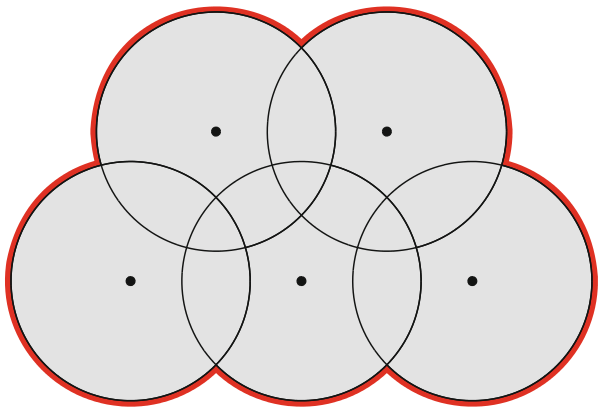
\includegraphics[width=.85\textwidth]{vdWS.png}
   \caption{\acrlong*{vdWS} (\acrshort{vdWS})}
   \label{fig:vdWS}
 \end{subfigure}
 ~
 \begin{subfigure}{.45\textwidth}
   \centering
   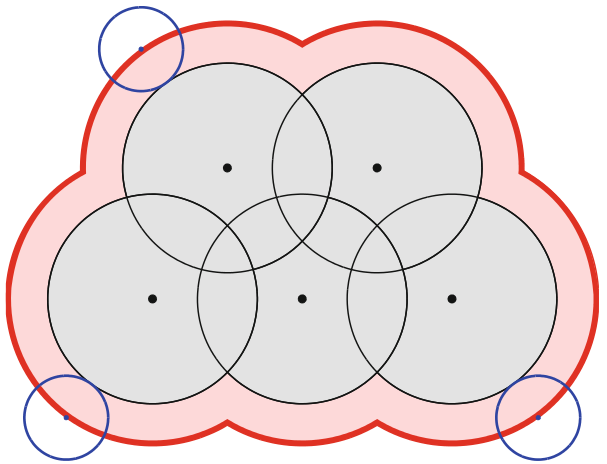
\includegraphics[width=.85\textwidth]{SAS.png}
   \caption{\acrlong*{SAS} (\acrshort{SAS})}
   \label{fig:SAS}
 \end{subfigure}

 \begin{subfigure}{.45\textwidth}
   \centering
   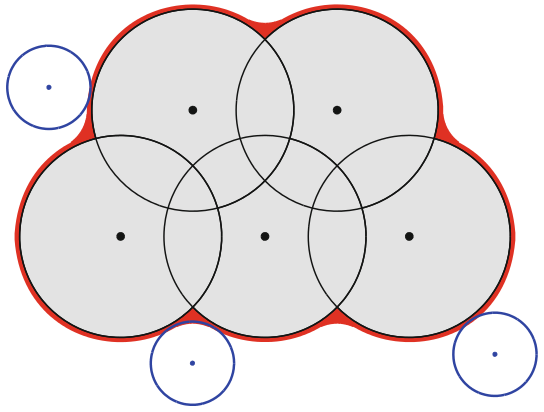
\includegraphics[width=.85\textwidth]{SES.png}
   \caption{\acrlong*{SES} (\acrshort{SES})}
   \label{fig:SES}
 \end{subfigure}
 \caption{Molecular surfaces from interlocking sets of atom-centered spheres.
 Reproduced from \noparcite[ref.][]{Harbrecht2011-dk}.}
\end{figure}
Alternative definitions based on the isodensity surface of the molecular solute
have been put forth.~\autocite{Foresman1996-wv}

Steps \ref{item:mesh} and \ref{item:discretize} are closely intertwined,
in the technical \acrshort{BEM} literature they go under the name of
\emph{finite element discretization}.
Let us define a mesh of the domain $\Gamma$ as an indexed collection of
intervals with non-zero measure $\lbrace I_i\rbrace_{i=1}^{N_\mathrm{mesh}}$, where
$N_\mathrm{mesh}$ is the size of the mesh.
Then, in a rather informal sense, a finite element is the
mathematical entity formed by the vector space of functions that are
piecewise regular on any given interval in the mesh.~\autocite{Ern2004-oo}
Basically, given an element in the mesh, we "attach" a basis set of
piecewise polynomials of a prescribed degree and use this basis to
provide a representation of quantities defined on $\Gamma$ within each
mesh interval.
Mesh generation for the molecular surfaces mentioned above is usually
achieved by modified triangulation procedures. In this thesis we used
the GePol algorithm~\autocite{Pascual-Ahuir1987-uo, Pascual-Ahuir1990-lp,
Pomelli1998-qp, Pomelli2001-sj, Frediani2004-ua, Pomelli2007-wq}
and the mesh generators of Harbrecht and Randrianarivony especially
tailored for the wavelet \acrshort{BEM}.~\autocite{Harbrecht2009-no,
Harbrecht2011-dk}

The finite element discretization is usually carried out either by the
\emph{collocation} or by the \emph{Galerkin} approach.
Indeed, it is possible to show that discretization by collocation
corresponds to a Galerkin method with a very specific (and asymmetric)
choice of \emph{trial} and \emph{test}
spaces.~\autocite{Hackbusch1995-uq, Ern2004-oo}
This step transforms the original integral equation into a system of
linear equations whose dimension relates to the underlying mesh size.
For general integral equations and finite element discretizations,
the \emph{stiffness matrix} obtained is dense and proper linear algebra
techniques need to be employed in order to avoid a detrimental impact on
computational performance.
In addition, finite element discretization might destroy intrinsic
symmetries of the original integral
operators. These can be recovered by appropriate \emph{a posteriori}
symmetrization procedures introducing, however, a degree of
arbitrariness in the \acrshort{BEM} procedure.~\autocite{Lange2011-eu}

In the GePol procedure, the molecular surface is meshed by means of
$N_\mathrm{ts}$ spherical polygons $\Pi_i$ whose centroids define the
collocation points. One-point quadrature rules are then applied at the
centroid to obtain the matrix equation:
\begin{equation}
 \mat{R}^{-1}\mat{T} \vect{q}
  =
  \vect{v}.
\end{equation}
$\vect{q}$ and $\vect{v}$ are vectors of dimension $N_\mathrm{ts}$
collecting the values of the \acrshort{ASC} and \gls{MEP}
at the collocation points. $\mat{R}^{-1}\mat{T}$ is the stiffness
matrix.
The matrices representing the boundary integral operators are:
\begin{align}
  \mat{T} &=
  \left(2\pi\mat{I} - \mat{D}_\mathrm{e}\mat{A}\right)\mat{S}_\mathrm{i}
  +\mat{S}_\mathrm{e}\left(2\pi\mat{I} +
  \mat{A}\mat{D}_\mathrm{i}^\dagger\right) \\
  \mat{R} &=
  \left(2\pi\mat{I} - \mat{D}_\mathrm{e}\mat{A}\right) -
  \mat{S}_\mathrm{e}\mat{S}^{-1}_\mathrm{i}\left(2\pi\mat{I}-\mat{D}_\mathrm{i}\mat{A}\right)
\end{align}
$\mat{I}$ is the $N_\mathrm{ts}$-dimensional identity matrix while the
other matrices are defined as:
\begin{subequations}
  \begin{align}
    A_{ij} &= a_i\delta_{ij}, \quad a_i = \mathrm{area}(\Pi_i) \\
    S_{ij, \mathrm{i}} &=
    k\sqrt{\frac{4\pi}{a_i}}\delta_{ij} +
    \frac{1}{|\vect{s}_i-\vect{s}_j|}(1-\delta_{ij}) \\
    D_{ii, \mathrm{i}} &=
    -k\sqrt{\frac{\pi}{a_i}}\frac{1}{R_i}\delta_{ij}
    + \frac{(\vect{s}_i-\vect{s}_j)\cdot\vect{n}_j}{|\vect{s}_i-\vect{s}_j|^3}(1-\delta_{ij})
  \end{align}
\end{subequations}
in terms of the centroids $\vect{s}_i, \vect{s}_j$, the finite elements
areas and their curvatures $R_i$.
The factor $k=1.07$ is introduced to achieve a better precision on the
diagonal elements.~\autocite{Tomasi2005-vm}
Expressions for $\mat{S}_\mathrm{e}$, $\mat{D}_\mathrm{e}$ and
$\mat{D}^\dagger_\mathrm{e}$ depend on the specific outer environment
and can be found in the literature.~\autocite{Corni2002-dr, Frediani2004-er,
Tomasi2005-vm, Delgado2013-kd, DiRemigio2016-nn}

The wavelet Galerkin \acrshort{BEM} was also used in this thesis. This method
preserves the fundamental symmetries of the boundary integral operators
and achieves sparsity in the stiffness matrix.
This sparsity can be leveraged to implement efficient algorithms with
linear space and time complexity. The approach is thus superior
to the traditional collocation method.

Given a hierarchical sequence of trial spaces
$\lbrace V_l\rbrace_{l=1}^J$, one can decompose the $l$-th element in
the hierarchy into the direct sum $V_l = V_{l-1} \oplus W_l$.
$W_l$ is called the \emph{wavelet space} and is the, not necessarily
orthogonal, complement to $V_{l-1}$.
Recursively applying this splitting to the trial spaces hierarchy
generates the wavelet decomposition, where all complementary spaces are
spanned by the wavelet basis.
The fundamental insight in the wavelet \acrshort{BEM} is to use the wavelet
basis for the discretization step and employ the compression technique
described by \citeauthor{Dahmen2006-pj} to build up the sparse system
matrix.~\autocite{Harbrecht2004-uo, Harbrecht2006-ug, Dahmen2006-pj}
Matrix compression is carried out in two rounds, \emph{a priori} and \emph{a
posteriori}, resulting in a finger-like sparsity pattern for the
stiffness matrix, Figure \ref{fig:finger-structure}.
The number of relevant matrix entries scales proportional to $O(N_J)$
with $N_J$ the number of degrees of freedom for a refinement of the
geometry up to level $J$.

\begin{figure}[tb]
   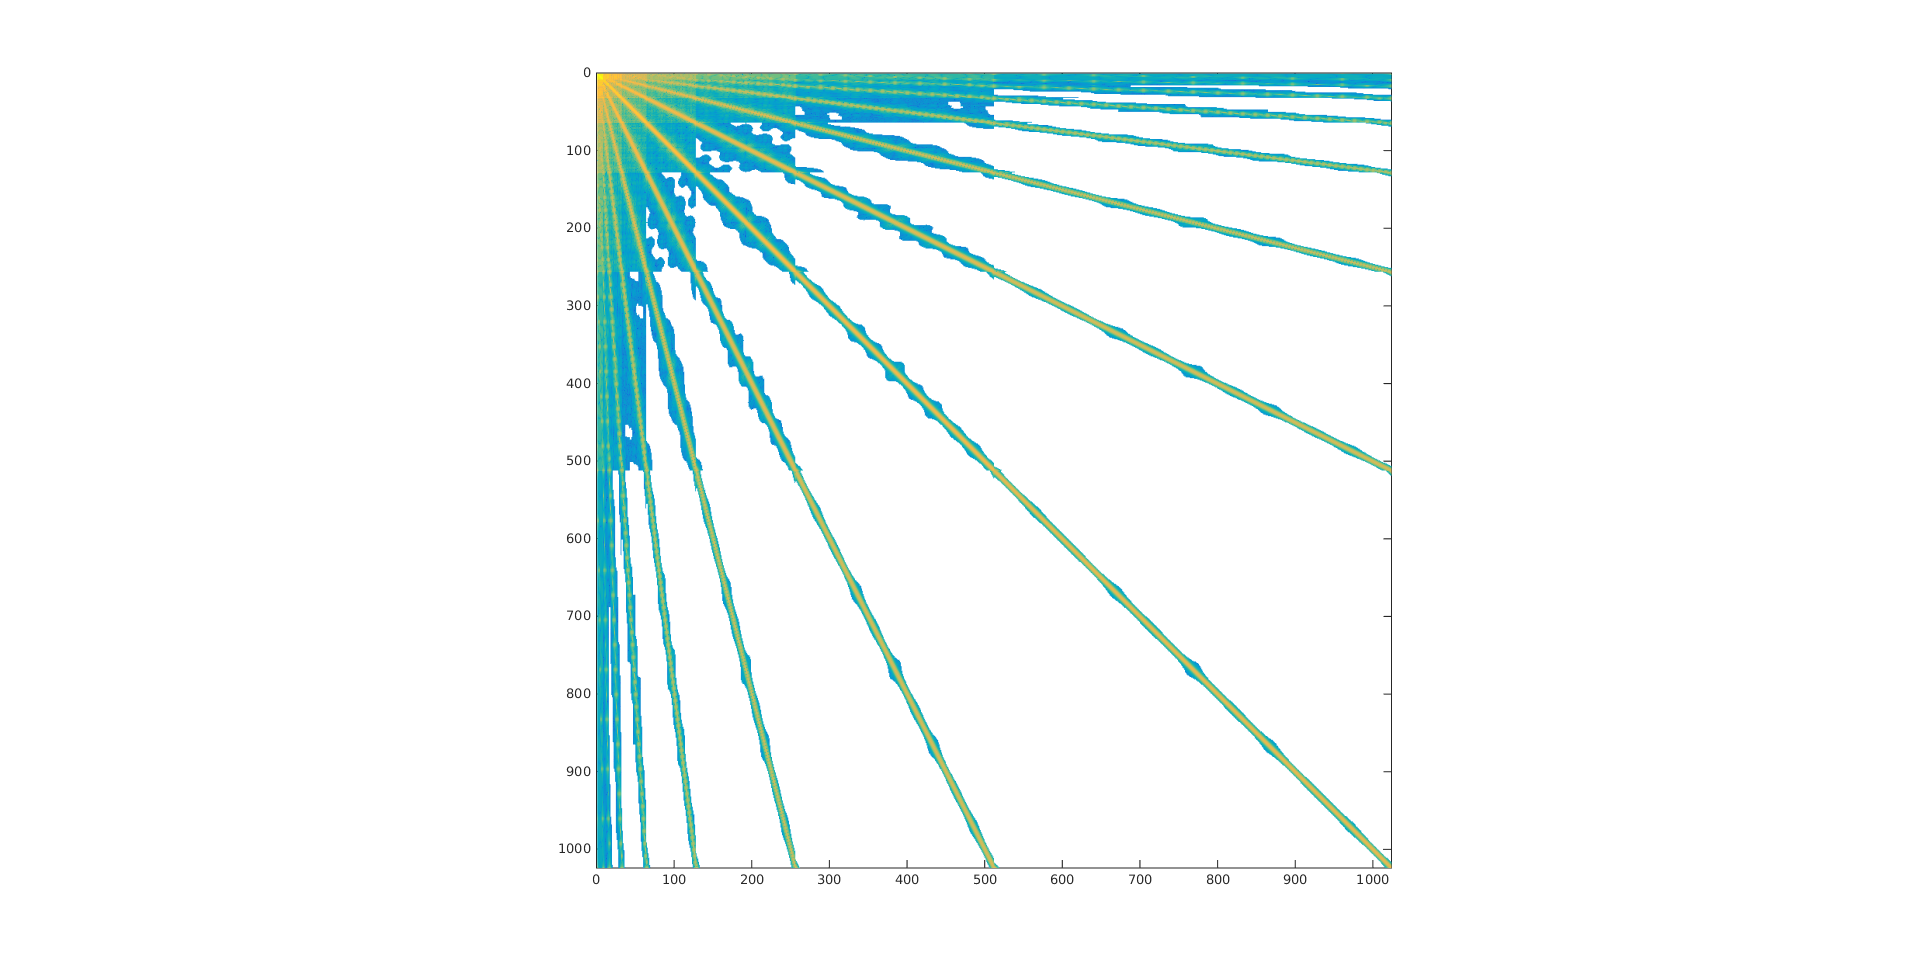
\includegraphics[width=\textwidth]{a_2_l_0_5_fs.png}
   \caption[Sparsity pattern achieved by the wavelet Galerkin \acrshort{BEM}.]{
   Sparsity pattern achieved by the wavelet Galerkin \acrshort{BEM} when
   solving the Laplace equation on 6 patches.
   Reproduced from \noparcite[ref.][]{Bugeanu2015-tp}.
   }
   \label{fig:finger-structure}
\end{figure}

Continuity of meshes with respect to molecular distortions is a
central issue for stable implementations of molecular gradients and
recurs frequently in the literature.
Numerous schemes have been proposed to solve or alleviate this issue.
We here mention the TsLess~\autocite{Pomelli2004-lb} and
DefPol~\autocite{Pomelli1998-ob, Pomelli1999-dc} approaches of
\citeauthor{Pomelli1998-ob} and the FIXPVA
modification~\autocite{Su2009-em} to the GePol algorithm put forth by
\citeauthor{Su2009-em}.
\citeauthor{Scalmani2010-tw} have recently proposed the \gls{CSC} scheme
which uses a smooth \acrshort{vdWS} and 3D spherical Gaussian basis
functions.~\autocite{Scalmani2010-tw, York1999-xy}
Gaussian blurring was also advocated by \citeauthor{Lange2010-jp} in
their \gls{SWIG} method.~\autocite{Lange2010-jp, Lange2010-qo}
Both \acrshort{CSC} and \acrshort{SWIG} achieve continuous \acsp{PES} and smooth
molecular gradients. However, their convergence to the exact solution of
the underlying integral equation has yet to be proved.
A completely different approach to the problem has been taken by
\citeauthor{Cances2013-jg} by employing a domain decomposition
method, guaranteed to converge to the exact solution.~\autocite{Quarteroni1999-jt}
Moreover, for \acrshort{COSMO}, the formulation is embarrassingly
parallel and has been implemented in a linearly scaling fashion.~\autocite{Cances2013-jg, Lipparini2013-cy, Lipparini2014-to,
Lipparini2014-fq}
Very recently the method has also been extended to general dielectric
environments.~\autocite{Stamm2016-fv}

In the following, the \acrshort{PCM} equations will be written in the
"complete basis" meaning that we will be working with the exact integral
equation and not with its discretized counterpart.
As a consequence, the apparent surface charge $\sigma$ and
the electrostatic potential $\esp$ will have a \emph{continuous}
dependence on a cavity surface "index" $\vect{s}$.
A product involving any of these quantities will have to be
interpreted as the \emph{surface integral}, \ie the scalar product in
the suitable, infinite-dimensional vector space on the cavity boundary
$\Gamma$.
The following shorthand notations will be adopted:
\begin{equation}
  \begin{aligned}
  \sigma\PCM\sigma &=
  \int_\Gamma\diff\vect{s}\sigma(\vect{s})\PCM\sigma(\vect{s})
  =
  \scalprod{\sigma}{\PCM\sigma} \\
  \sigma\esp &=
  \int_\Gamma\diff\vect{s}\sigma(\vect{s})\esp(\vect{s})
  =
  \scalprod{\sigma}{\esp}
  \end{aligned}
\end{equation}

\section[Variational Formulation of Classical Polarizable Models]{
Variational Formulation of Classical Polarizable Models}
\label{sec:variational}

The attentive reader will have noticed that, despite the focus of this
thesis on continuum models for the quantum mechanical modelling of
solvation, no mention has been made so far in this Chapter of any
quantum aspect.
The strategy usually adopted is to tailor a specific Hamiltonian, which
includes classical contributions form the continuum and use it in the
development of the quantum chemical model.
Since the \acrshort{MEP} is a linear functional of the solute charge density,
the \acrshort{ASC} itself incurs in a dependency on the solute charge
density.
Properly accounting for the mutual solute-solvent polarization induces a
\emph{nonlinearity} in an otherwise linear problem.
Manipulating such a \emph{nonlinear} Schr\"{o}dinger equation is
theoretically cumbersome,\autocite{Sanhueza1979-bp, Heimsoeth1990-ki}
but has been successfully exploited in the past.\autocite{Tomasi2005-vm}

In this thesis we advocate a different theoretical approach: the
variational formulation of classical polarizable models.
Why so? In such a framework the \acrshort{ASC} becomes an additional,
independent, variationally optimizable degree of freedom.
This makes the coupling to, \eg, extended Lagrangian dynamics
trivial.\autocite{Car1985-jw}
It is well known that electrodynamics can be derived as the minimization
of an action functional.\autocite{Jackson1999}
The principle of least action is however formulated in terms of
\emph{fields} and not more easily manageable quantities, such as the
\acrshort{MEP} or the \acrshort{ASC}.
A true energy functional has to fulfill the following
properties:\autocite{Solis2013-ef}
\begin{enumerate*}[label={\alph*)},font={\color{PMS1797}}]
    \item physical extremal points,
    \item equilibrium values are true energies \label{item:equil-prop} and
    \item convexity (positive-definiteness)
\end{enumerate*}
\citeauthor{Allen2001-fp} and \citeauthor{Attard2003-vr} pioneering
attempts resulted in functionals of scalar densities violating
Property \ref{item:equil-prop} and could not thus be used in extended Lagrangian
dynamics.\autocite{Allen2001-fp, Attard2003-vr, Attard2007-lk}

In a seminal paper, \citeauthor{Lipparini2010-be} showed how the
\acrshort{PCM} can be recast in a variational fashion yielding a true energy
functional of the \acrshort{ASC}:\autocite{Lipparini2010-be, Lipparini2011-aj, Lipparini2016-mo}
\begin{equation}\label{eq:pcm-functional}
 U_\mathrm{PCM} = \frac{1}{2}\sigma\PCM\sigma + \esp\sigma,
 \quad
  \PCM = \bi{R}_\infty^{-1}\bi{R}_\diel\bi{S}.
\end{equation}
yielding Eq.~\eqref{eq:isotropic-IEF} upon minimization:
\begin{equation}\label{eq:pcm-stationarity}
  \pderiv{U_\mathrm{PCM}}{\sigma} = \PCM\sigma + \varphi = 0.
\end{equation}
It is interesting to note how this functional follows quite immediately
from the integral equation formulation and standard results in the
theory of boundary integral equations.\autocite{Hsiao2008-xb}

Explicit classical polarizable models can also be recast in a
variational fashion allowing for their treatment on par with implicit
classical polarizable models.
The functional looks as follows:
\begin{equation}\label{eq:mm-functional}
  U_\mathrm{MM} = \frac{1}{2}\kappa\MM\kappa + \kappa\zeta,
\end{equation}
here $\kappa$ is the variational degree of freedom representing
the polarization of the explicit environment. $\zeta$ is the inducing
field, \emph{vide infra}. The reader is referred to the works of
\citeauthor{Lipparini2011-rd} for a derivation of this functional.\autocite{Lipparini2011-rd, Lipparini2015-lq, Loco2016-oy}
We have made no specific reference to the particular explicit
model used. The variational framework is flexible enough to encompass
either the MMpol,\autocite{Mennucci2013-go}
the \gls{PE},\autocite{Olsen2010-wa, Olsen2011-io} or
the \gls{FQ} model.\autocite{Rick1994-mn, Rick1995-wu, Rick1996-om,
Lipparini2011-rd}

Coupling the implicit and explicit polarizable models is straightforward
in the variational framework:\autocite{Steindal2011-ki, Lipparini2011-rd,
Caprasecca2012-ir, Lipparini2013-ud}
\begin{equation}\label{eq:pcm-mm-functional}
  U_\mathrm{pol} =
   \frac{1}{2}\sigma\PCM\sigma + \sigma\esp
 + \frac{1}{2}\kappa\MM\kappa + \kappa\zeta
 + \sigma\bi{X}\kappa.
\end{equation}
An additional term, as first derived by
\citeauthor{Steindal2011-ki},\autocite{Steindal2011-ki} was added to
account for the mutual polarization between the implicit and explicit
layers:
\begin{equation}
  \sigma\MMPCM\kappa = \kappa\MMPCM^\dagger\sigma
\end{equation}
$\MMPCM$ is the implicit/explicit interaction kernel, whose form depends
on the specific explicit model chosen.

The global minimum of the convex functional is found by differentiating
with respect to the variational degrees of freedom:
\begin{equation}\label{eq:pcm-mm-stationarity}
  \begin{pmatrix}
    \PCM & \MMPCM \\
    \MMPCM^\dagger & \MM
  \end{pmatrix}
  \begin{pmatrix}
   \sigma \\
   \kappa
  \end{pmatrix}
  =
  -
  \begin{pmatrix}
   \esp \\
   \zeta
  \end{pmatrix}
\end{equation}
While $\esp$ is quite clearly the \acrshort{MEP}, $\zeta$ can either be the
molecular electric field (MMpol and \acrshort{PE} models) or again the
\acrshort{MEP} (\acrshort{FQ} model).
In any case, both will be determined by the quantum mechanical molecular
charge density and can thus be formulated as expectation values of
one-electron operators.
Eventually, this achieves the coupling between the classical -- $\sigma$
and $\kappa$ -- and the quantum mechanical variational degrees of
freedom.

The functionals in Eqs.~\eqref{eq:pcm-functional},
\eqref{eq:mm-functional} and \eqref{eq:pcm-mm-functional} all have a
clear physical meaning.
They describe charge distributions interacting (unfavorably) with
themselves and (favorably) with their respective inducing external
fields and constitutes the polarization energy of the medium.
The topic of variational formulations is particularly important in the
field of \acrshort{MD} simulations.\autocite{Jadhao2012-gf, Jadhao2013-ry, Jadhao2013-hs,
Solis2013-ef}
Our focus however is on the quantum mechanical calculations of molecular
properties and the variational formulation is advantageous since it
dispenses us from manipulating cumbersome nonlinear coupling terms in
the Hamiltonian.
Moreover, the stationarity condition Eq.~\ref{eq:pcm-mm-stationarity}
entails the existence of a classical Hellmann--Feynman theorem:
\begin{equation}\label{eq:classical-HF}
  \deriv{U_\mathrm{pol}}{F} = \pderiv{U_\mathrm{pol}}{F}
  + \pderiv{U_\mathrm{pol}}{\sigma}\pderiv{\sigma}{F}
  + \pderiv{U_\mathrm{pol}}{\kappa}\pderiv{\kappa}{F}
  = \pderiv{U_\mathrm{pol}}{F},
\end{equation}
which is paramount in the formulation of molecular properties, see
Chapter \ref{ch:molprop}.
The variational formulation also lends itself to an implementation
in terms of simultaneous optimization.\autocite{Lipparini2011-aj}

Finally, let us re-express the equations above in a supermatrix
formalism:
\begin{equation}\label{eq:supermatrix-functional}
  U_\mathrm{pol} =
  \frac{1}{2}{}^t\p\V\p + {}^t\p\s
\end{equation}
where:
\begin{alignat}{3}
  \p =
  \begin{pmatrix}
    \sigma \\
    \kappa
  \end{pmatrix},
  \quad&
  \s =
  \begin{pmatrix}
   \esp \\
   \zeta
  \end{pmatrix},
  \quad&
  \V =
  \begin{pmatrix}
    \PCM & \MMPCM \\
    \MMPCM^\dagger & \MM
  \end{pmatrix}
\end{alignat}
and the ${}^t\p$ symbol denotes the transposed supervector $\p$.
The scalar products are understood to be in the relevant function
spaces.
The supermatrix formalism will be adopted throughout the thesis.

How are quantum/classical polarizable Hamiltonians implemented in this
framework?
As shown in Chapter \ref{ch:QM} for the \acrshort{CC} method, one can
formulate methods in quantum chemistry as the unconstrained minimization
of a Lagrangian.
Due to the  variational property of the classical polarizable functional
one can devise an \emph{effective} quantum/classical polarizable
Lagrangian:\autocite{Lipparini2016-mo}
\begin{equation}
  \mathcal{L}_\mathrm{eff}(\vect{\eta}, \bar{\vect{\eta}}, \p) =
  \mathcal{L}(\vect{\eta}, \bar{\vect{\eta}}) +
  \frac{1}{2}{}^t\p\V\p + {}^t\p\s(\vect{\eta}, \bar{\vect{\eta}})
\end{equation}
and derive the governing equations in the usual manner:
\begin{subequations}
  \begin{align}
    \pderiv{\mathcal{L}_\mathrm{eff}(\vect{\eta}, \bar{\vect{\eta}}, \p)}{\bar{\vect{\eta}}}
    &= \mat{\Omega}(\vect{\eta}) + {}^t\p\pderiv{\s(\vect{\eta}, \bar{\vect{\eta}})}{\bar{\vect{\eta}}} = 0 \\
    \pderiv{\mathcal{L}_\mathrm{eff}(\vect{\eta}, \bar{\vect{\eta}}, \p)}{\vect{\eta}}
    &= \pderiv{\mathcal{E}(\vect{\eta})}{\vect{\eta}} +
    \scalprod[W]{\bar{\vect{\eta}}}{\pderiv{\mat{\Omega(\vect{\eta})}}{\vect{\eta}}}
    + {}^t\p\pderiv{\s(\vect{\eta}, \bar{\vect{\eta}})}{\vect{\eta}}
    = 0 \\
    \pderiv{\mathcal{L}_\mathrm{eff}(\vect{\eta}, \bar{\vect{\eta}}, \p)}{\p} &=
    \V\p + \s(\vect{\eta}, \bar{\vect{\eta}}) = 0
  \end{align}
\end{subequations}
The quantum mechanical and the classical model are thus fully coupled,
due to the dependence of the source term $\s$ on the amplitudes and
multipliers.

As an example, let us consider the single-reference \acrshort{HF} and
\acrshort{KS}-\acrshort{DFT} methods introduced in Section
\ref{sec:mean-field}.
First of all, we need the appropriate \acrshort{SCF} energy functional
\emph{in vacuo}.
The \acrshort{AO} basis set expansion of the \glspl{MO} lets us define
the one-electron \acrshort{AO} density matrix as:
\begin{equation}
  D_{\mu\nu} = \sum_{i=1}^{N_O}C_{\mu i}C^\dagger_{\nu i}
\end{equation}
where $C_{\alpha r}$ are the \acrshort*{MO} expansion coefficients and
$N_O$ is the total number of occupied orbitals.
The \acrshort*{SCF} energy functional \emph{in vacuo} can now be
expressed as:
\begin{equation}\label{eq:scf-functional}
  \mathcal{E}(\mat{C}) \eqtr \mat{h}\mat{D} + \frac{1}{2}
  \mat{G}^\gamma(\mat{D})\mat{D} + E_\mathrm{xc}[\rho(\vect{r})] +
  V_\mathrm{NN},
\end{equation}
and has to be optimized under the \acrshort*{MO} orthonormality
constraint, easily introduced by means of Lagrangian multipliers:
\begin{equation}\label{eq:scf-lagrangian}
  \mathcal{L}(\mat{C}, \mat{\epsilon}) = \mathcal{E}(\mat{D}) -
  \sum_{ij}\epsilon_{ji}(\braket{\phi_i|\phi_j} - \delta_{ij})
\end{equation}
The various contributions are expressed in terms of \acrshort*{AO} basis
integral and density matrices:
\begin{subequations}
  \begin{align}
  h_{\mu\nu} = &= \int \diff\vect{r}
  \chi_\mu^\dagger(\vect{r})h(\vect{r})\chi_\nu(\vect{r}) \label{eq:ao-one-el} \\
  G_{\mu\nu}^\gamma &=
  \sum_{\kappa\lambda}D_{\kappa\lambda}(g_{\mu\nu\kappa\lambda} -
  \gamma g_{\mu\lambda\kappa\nu}) \label{eq:two-el-matrix} \\
  g_{\mu\nu\kappa\lambda} &=
  \int\diff\vect{r}\int\diff\vect{r}^\prime
  \Omega_{\mu\nu}(\vect{r}) g(\vect{r},\vect{r}^\prime)
  \Omega_{\kappa\lambda}(\vect{r}^\prime) \label{eq:ao-two-el} \\
  E_\mathrm{xc}[\rho(\vect{r})] &=
  \int\diff\vect{r}
  v_\mathrm{xc}(\vect{r})\Tr\mat{\Omega}(\vect{r})\mat{D} \label{eq:ao-xc} \\
  \Omega_{\mu\nu}(\vect{r}) &= \chi_\mu^\dagger(\vect{r})\chi_\nu(\vect{r}).
  \label{eq:ao-overlap}
  \end{align}
\end{subequations}
The quantum/classical polarizable \acrshort*{SCF} functional is obtained by adding the
polarization functional to Eq. \eqref{eq:scf-functional}:
\begin{equation}\label{eq:polarizable-scf-functional}
  \mathcal{L}_\mathrm{eff}(\mat{C}, \mat{\epsilon}, \s) =
  \mathcal{L}(\mat{C}, \mat{\epsilon}) +
  \frac{1}{2}{}^t\p\V\p + {}^t\p\Tr\mathbfup{s}\mat{D}.
\end{equation}
Differentiation with respect to the variational degrees of freedom
yields the \acrshort*{KS} and polarization equations:
\begin{subequations}
  \begin{align}
    \mat{F}\mat{C} &= \mat{S}\mat{C}\mat{\epsilon} \\
    \V\p &+ \Tr\mathbfup{s}\mat{D} = 0 \label{eq:polarization-stat}
  \end{align}
\end{subequations}
The \acrshort*{KS} matrix now includes environment contributions:
\begin{equation}
  f_{\mu\nu} = h_{\mu\nu}  + G^\gamma_{\mu\nu}(\mat{D}) + f_{\mathrm{xc};\mu\nu}
  + {}^t\p\s_{\mu\nu}.
\end{equation}
With respect to the coupling described in abstract terms above, the
\acrshort*{SCF} case is formally simpler. In fact, whereas in the
general case the source term depends on \emph{both} primal (amplitudes)
and dual (multipliers) variational degrees of freedom, here only the
dependence on the primal parameters (\acrshort*{MO} coefficients) needs
to be considered.\autocite{Lipparini2011-aj}
